\documentclass[preprint,12pt,3p]{elsarticle}

\usepackage{amsmath}
\usepackage{amssymb}
\usepackage{bbm}
\usepackage{graphicx}
\usepackage{sidecap}
\usepackage{url}
\usepackage{algpseudocode}
\usepackage{amsthm}

\DeclareMathOperator{\sign}{sign}
\DeclareMathOperator{\proj}{proj}

\geometry{bottom=2.5cm, top=2.5cm}
\footskip 1.3cm

\allowdisplaybreaks

\begin{document}

% Title


\centering

\Large Predicting Gaze Direction via Convolutional Neural Networks\\\large Project: MATVMD861, WiSe 2016-2017\\\bigskip\bigskip

\normalsize Chris Kindler
\\
\bigskip\bigskip\bigskip


% Main


\justify
% \addtocounter{section}{-5}

% Abstract

\hrule
\bigskip
\textbf{Abstract}
\smallskip

\noindent
In the following we will discuss the application of convolutional neural networks (ConvNets) as a tool to predict the gaze direction of a person given an image of their head. We first give a short overview of classification and regression with simple artificial neural networks and explain the general principles involved in the learning process. After that we discuss some more sophisticated architectures and go into some detail examining different learning algorithms and their application in neural networks. We continue by taking a closer look at ConvNets, exploring the different types of layers used and considering some of the intricacies involved in constructing properly functioning convolutional networks. Following that we present the implementation of a small number of networks trained on the data and compare the results to those achieved by different machine learning approaches. We end by discussing some real world scenarios in which the task of predicting gaze direction or a variation thereof could find relevance and trying to evaluate the viability of our models.
\\
\medskip
\hrule
\bigskip
\bigskip
\bigskip

% Section 1

\section{Artificial Neural Networks}

Neural networks have, in the last decade, become an exceedingly popular tool employed to approach classification as well as regression problems across various domains \cite{goossens93}. The basis of these networks is made up by a large number of basic computation units, so called 'neurons', every one of which takes a number of weighted signals as an input, processes them and outputs a new signal. These neurons are then connected in various ways to pass information from a initial input to a final output, i.e. the network part of neural network. The name is originally derived from processes involved in information processing in the human brain and even though we by now know that this comparison grossly understates the complexity of the brain and its inner workings, it is still a convenient analogy to give some insight into how artificial neural networks function at a lower level (See Figure \ref{fig:ANNs}). 

If we want a higher level description we will need to concentrate on a specific type of architecture since different architectures can vary quite heavily in their structure. Since we do not want to spend excessive amounts of time on this topic and because from a pedagogical standpoint it makes sense to open up with something plain and easily understandable, we will start by taking a closer look at one of, if not the simplest neural network archetypes, feedforward neural networks or 'Multilayer Perceptron', and then give a rather brief overview of the multitude of variations and alternatives that have been developed.



\subsection{Multilayer Perceptron}

\begin{figure}
    \centering
    \hspace*{-1.5cm}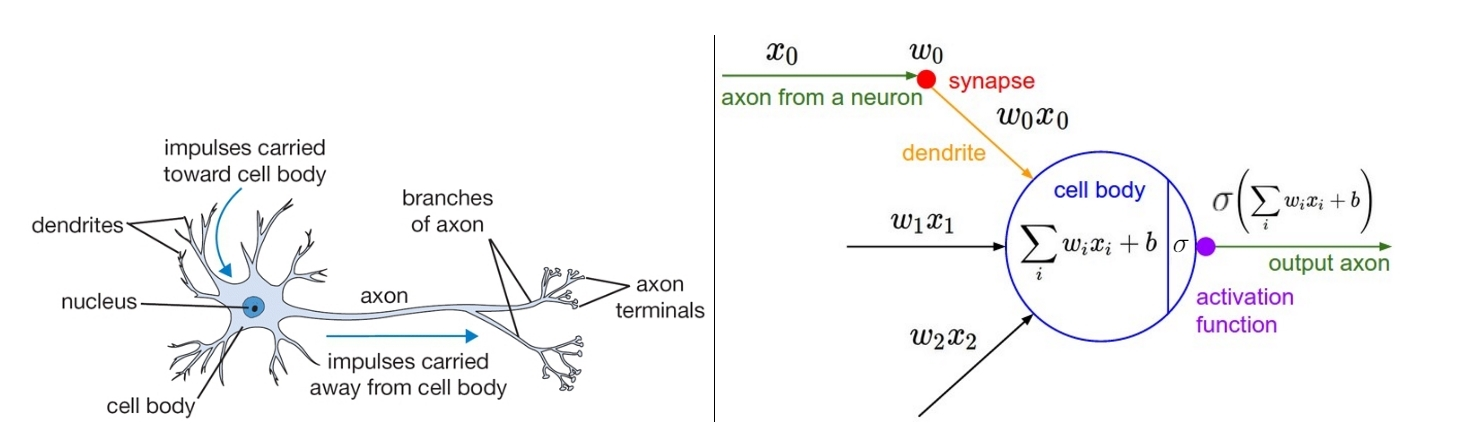
\includegraphics[scale=0.5]{figures/ANNs}
    \caption{A cartoon drawing of a biological neuron (left) and its mathematical model (right) \cite{Xmisc}}
    \label{fig:ANNs}
\end{figure}

Our first step on the way to understand simple neural networks will be to recall the perceptron algorithm (A short recap can be found in Appendix A). In Perceptron, as in all linear classification methods, a labeled dataset 
$${\mathcal{D}=\{(\mathbf{x}^i,y^i)\in\mathbb{R}^d\times\{0,1\}\,|\,i=1,...,n\}}$$ 
is used to train the classifier in the following way. For each data point $x^i$ we calculate 
$$\alpha^i=\sum_{j=1}^dx^i_jw_j+b$$
for weights $\mathbf{w}$ and bias $b$, then output 
\begin{align*}
    \sigma(\alpha^i)=\begin{cases}0 &\mbox{if }\alpha^i<0\\
    1 & \mbox{otherwise}\end{cases}
\end{align*} 
and finally we can compare the output to the label with some loss, e.g.
$$\mathcal{L}(\mathbf{w},b;\mathcal{D})=\sum_{i=1}^n(y^i-\sigma(\alpha^i))^2$$
We can see that this has a lot in common with the mathematical model of a single neuron seen in Fugure \ref{fig:ANNs}. The neuron gets weighted signals $w_jx_j$, processes them ${\alpha=\sum_{j=1}^dw_jx_j+b}$ and outputs a new signal $\sigma(\alpha)$. Theoretically we could now begin stacking up these neurons into layers, connecting the layers (See \ref{fig:ANNs2}) and thus create networks only containing these very simple perceptron neurons. It turns out however that only being able to send out binary signals severely constrains the ability of a network which is why we will try to find another, better suited option. Our options here are plentiful, but the one used most commonly in multilayer perceptron is the sigmoid function
$$\sigma(x)=\frac{1}{1+e^{-x}}$$
This function is used heavily for two main reasons. For one, it is a smooth approximation of the Heaviside step function, which makes it differentiable while still being easily interpretable. And secondly its derivative is given by
\begin{align*}
    \frac{d}{dx}\sigma(x)&=\frac{d}{dx}\Big(\frac{1}{1+e^{-x}}\Big)\\
    &=e^{-x}\Big(\frac{1}{(1+e^{-x})^2}\Big)\\
    &=\Big(\frac{e^{-x}}{1+e^{-x}}\Big)\Big(\frac{1}{1+e^{-x}}\Big)\\
    &=(1-\sigma(x))\sigma(x)
\end{align*}
the enormous use of which we will see a bit later on when we discuss the learning algorithm. 
As a small aside, using a single neuron with sigmoid activation is also known as logistic regression .
\begin{figure}
    \centering
    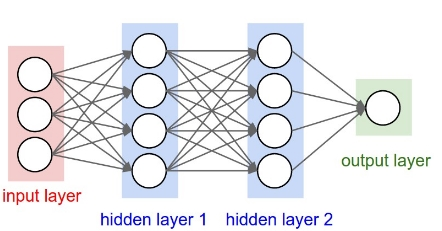
\includegraphics[scale=1]{figures/ANNs2}
    \caption{A 3-layer neural network with three inputs, two hidden layers of 4 neurons each and one output layer \cite{Xmisc}}
    \label{fig:ANNs2}
\end{figure}

So now that we have all the parts and some intuition we can formally introduce multilayer perceptron. Let $L\in\mathbbm{N}$ be the number of layers (L-1 hidden layers and one output layer) in the network and $N_l\in\mathbbm{N}$ the number of neurons in each layer. For a data point $\mathbf{x}\in\mathbbm{R}^n$ we define
\begin{align*}
    &x^0_i=x_i & x^l_i=\sigma\Big(\sum_{j=1}^{N_{l-1}}w^{l}_{i,j}x^{l-1}_j+b^{l}_i\Big)
\end{align*}
As before we use the shorthand $\alpha^l_i=\sum_{j=1}^{N_{l-1}}w^{l}_{i,j}x^{l-1}_j+b^{l}_i$ so that $x^l_i=\sigma(\alpha^l_i)$. For instance the signals, that the first hidden layer outputs are given by
\begin{align*}
    x^1_i=\sigma(\alpha^1_i)=\sigma\Big(\sum_{j=1}^{N_{l-1}}w^1_{i,j}x_j+b^1_i\Big)
\end{align*}
and we predict $\hat{y}(\mathbf{x};\mathbf{w},\mathbf{b})=g(\mathbf{x}^L)$. With $\mathbf{w}$ and $\mathbf{b}$ we simply denote the complete collection of weights and bias terms in the network. 

As an example imagine a classification problem with $K$ classes. A typical approach to design a network for such a problem would be to use $K$ output neurons and interpret the results in the $k$-th neuron as a score for class $k$, so that 
$$\hat{y}(\mathbf{x};\mathbf{w},\mathbf{b})=arg\max_{k\in\{1,...,K\}}(x_k^L)$$
What we can observe is that in multilayer perceptron information is only ever directly passed forward from the $l$-th layer to the $l+1$-th, which is why these networks are also called feedforward neural networks. On one hand this certainly leads to conceptualizing these networks being a lot easier and some learning methods almost being straightforward, as we will see in a moment. But on the other hand, removing these restrictions allows for network architectures that have been shown to be hugely effective in certain paradigms. some of which we will touch on a bit later on.

\subsection{Backpropagation}

As with architectures, there is a plethora of learning approaches designed for neural networks and again as with architectures we shall explore one in some detail and name a few others down the line. But before we begin, we will need some more notation. Firstly by $E(\mathbf{x}^L,y)$ we denote some error function between the real and the predicted label. This could for example be the (multiclass) hinge loss
$$E(\mathbf{x}^L,\mathbf{y})=\sum_{k\neq y}\max(0,x^L_k-x^L_y+\Delta)$$
with some hyper parameter $\Delta$ or cross entropy loss
$$E(\mathbf{x}^L,\mathbf{y})=-\log\Big(\frac{\exp(x^L_y)}{\sum_{k=1}^K\exp(x_k^L)}\Big)$$
Secondly, what we will try to understand here is a single update of the parameters from $(\mathbf{w}^{old},\mathbf{b}^{old})$ to $(\mathbf{w}^{new},\mathbf{b}^{new})$. Because there are three indeces on $w^l_{i,j}$ already, for readability it would probably be best to not keep plastering it with more which is why we will use the shorthand $(\tilde{\mathbf{w}},\tilde{\mathbf{b}})$ for the new parameters and just use $(\mathbf{w},\mathbf{b})$ for the old ones.

So assume we have a feedforward neural network with parameters $(\mathbf{w},\mathbf{b})$ and want to update it according to a new labeled data point $(\mathbf{x},y)$. One way to do this is by taking a single gradient step with respect to the relevant parameters with some learning rate $\eta$. For the weights in the last layer this would look as follows.
\begin{align*}
    \tilde{w}^L_{n,j}&=w^L_{n,j}-\eta\frac{\partial}{\partial w^L_{n,j}}E(\mathbf{x}^L,y)
\end{align*}
with $\frac{\partial}{\partial w^L_{n,j}}E(\mathbf{x}^L,y)$ being the interesting term. By chain rule we know that
\begin{align*}
    \frac{\partial}{\partial w^L_{n,j}}E(\mathbf{x}^L,y)&=\langle\frac{\partial}{\partial w^L_{n,j}}\mathbf{x}^L,\nabla_{\mathbf{x}^L}E(\mathbf{x}^L,y) \rangle\\
    &=\sum_{k=1}^{N_L}\Big(\frac{\partial}{\partial w^L_{n,j}}x^L_k\Big)\Big(\frac{\partial}{\partial x^L_k}E(\mathbf{x}^L,y)\Big)\\
    &=\sum_{k=1}^{N_L}\Big(\frac{\partial}{\partial w^L_{n,j}}\sigma(\alpha^L_k)\Big)\Big(\frac{\partial}{\partial x^L_k}E(\mathbf{x}^L,y)\Big)\\
    &=\sum_{k=1}^{N_L}\Big(\frac{\partial}{\partial w^L_{n,j}}\alpha_k^L\Big)\sigma'(\alpha^L_k)\Big(\frac{\partial}{\partial x^L_k}E(\mathbf{x}^L,y)\Big)\\
    &=\sum_{k=1}^{N_L}\Big(\frac{\partial}{\partial w^L_{n,j}}\sum_{i=1}^{N_{L-1}}(x^{L-1}_iw^L_{i,k}+b^L_k)\Big)\sigma'(\alpha^L_k)\Big(\frac{\partial}{\partial x^L_k}E(\mathbf{x}^L,y)\Big)\\
    &=\sum_{k=1}^{N_L}\sum_{i=1}^{N_{L-1}}\Big(\frac{\partial}{\partial w^L_{n,j}}(x^{L-1}_iw^L_{i,k}+b^L_k)\Big)\sigma'(\alpha^L_k)\Big(\frac{\partial}{\partial x^L_k}E(\mathbf{x}^L,y)\Big)\\
    &=\sum_{k=1}^{N_L}\sum_{i=1}^{N_{L-1}}\Big(1_{\{i=n,j=k\}}x^{L-1}_i)\Big)\sigma'(\alpha^L_k)\Big(\frac{\partial}{\partial x^L_k}E(\mathbf{x}^L,y)\Big)\\
    &=x^{L-1}_n\sigma'(\alpha^L_j)\frac{\partial}{\partial x^L_j}E(\mathbf{x}^L,y)
\end{align*}
If we take the specific example of sigmoid activation function and cross entropy loss we get the update step
\begin{align*}
    \tilde{w}^L_{n,j}&=w^L_{n,j}-\eta x^{L-1}_n\sigma(\alpha^L_j)(1-\sigma(\alpha^L_j))\Big(-1_{\{y=j\}}+\frac{\exp(x^L_j)}{\sum_{k=1}^K\exp(x_k^L)}\Big)\\
    &=w^L_{n,j}-\eta x^{L-1}_nx^L_j(1-x^L_j)\Big(-1_{\{y=j\}}+\frac{\exp(x^L_j)}{\sum_{k=1}^K\exp(x_k^L)}\Big)
\end{align*}
since, as mentioned above, for the sigmoid function we have $\sigma'(\alpha)=\sigma(\alpha)(1-\sigma(\alpha))$ and cross entropy loss can be rewritten in the following way
\begin{align*}
    -\log\Big(\frac{\exp(x^L_y)}{\sum_{k=1}^K\exp(x_k^L)}\Big)=-x^L_y+\log(\sum_{k=1}^K\exp(x_k^L))
\end{align*}
which makes it relatively easy to see, that its partial derivative with respect to $x^L_j$ is given by 
$$-1_{\{y=j\}}+\frac{\exp(x^L_j)}{\sum_{k=1}^K\exp(x_k^L)}$$
It is equally easy to see that the update step for $b_j^L$ is given by
\begin{align*}
    \tilde{b}^L_{j}&=b^L_{j}-\eta\sigma'(\alpha^L_j)\frac{\partial}{\partial x^L_j}E(\mathbf{x}^L,y)\\
    &=b^L_{j}-\eta x^L_j(1-x^L_j)\Big(-1_{\{y=j\}}+\frac{\exp(x^L_j)}{\sum_{k=1}^K\exp(x_k^L)}\Big)
\end{align*}
So now that we have the update steps, and more importantly the partial derivatives with respect to the signals $x_j^L$ in the last layer we can use that knowledge to calculate updates for the next to last layer. More generally we can calculate partial derivatives in layer $l$ given those in layer $l+1$ in the following way.
Let $\delta_k^{l}=\frac{\partial}{\partial x^{l}_k}E(\mathbf{x}^L,y)$
\begin{align*}
    \frac{\partial}{\partial w^l_{n,j}}E(\mathbf{x}^L,y)
    &=\langle\frac{\partial}{\partial w^l_{n,j}}\mathbf{x}^l,\nabla_{\mathbf{x}^l}E(\mathbf{x}^L,y) \rangle\\
    &=\sum_{k=1}^{N_l}\Big(\frac{\partial}{\partial w^l_{n,j}}x^l_k\Big)\Big(\frac{\partial}{\partial x^l_k}E(\mathbf{x}^L,y)\Big)\\
    &=x^{l-1}_n\sigma'(\alpha^l_j)\frac{\partial}{\partial x^l_j}E(\mathbf{x}^L,y)\\
    &=x^{l-1}_n\sigma'(\alpha^l_j)\delta_j^{l}
\end{align*}
meaning we have to find $\delta_j^{l}=\frac{\partial}{\partial x^l_j}E(\mathbf{x}^L,y)$. But again we can use the chain rule and get
\allowdisplaybreaks
\begin{align*}
    \frac{\partial}{\partial x^l_j}E(\mathbf{x}^L,y)&=\langle\frac{\partial}{\partial x^l_j}\mathbf{x}^{l+1},\nabla_{\mathbf{x}^l}E(\mathbf{x}^L,y) \rangle\\
    &=\sum_{k=1}^{N_{l+1}}\Big(\frac{\partial}{\partial x^l_j}x^{l+1}_k\Big)\Big(\frac{\partial}{\partial x^{l+1}_k}E(\mathbf{x}^L,y)\Big)\\
    &=\sum_{k=1}^{N_{l+1}}\Big(\frac{\partial}{\partial x^l_j}\sigma(\alpha_k^{l+1})\Big)\delta^{l+1}_k\\
    &=\sum_{k=1}^{N_{l+1}}\Big(\frac{\partial}{\partial x^l_j}\sum_{i=1}^{N_l}w_{i,k}^{l+1}x_i^l+b_k^{l+1}\Big)\sigma'(\alpha_k^{l+1})\delta^{l+1}_k\\
    &=\sum_{k=1}^{N_{l+1}}w_{j,k}^{l+1}\sigma'(\alpha_k^{l+1})\delta^{l+1}_k\\
\end{align*}
This is a recurrent rule to, given $\boldsymbol{\delta}^{l+1}$, calculate $\boldsymbol{\delta}^{l}$ which is all we need to update $w^l_{n,j}$ and similarly $b^l_{j}$. 
So to reiterate, the update process has the following steps:

\smallskip
Step 1: Find $\delta_j^{L}=\frac{\partial}{\partial x^{L}_j}E(\mathbf{x}^L,y)$

Step 2: Iterate over $l$ from $L$ to 1 and update  
\begin{align*}
    \tilde{w}^l_{n,j}  &=w^l_{n,j}-\eta x_n^{l-1}\sigma'(\alpha^l_j)\delta_j^{l}\\
    \tilde{b}^l_{j}\phantom{al}    &=b^l_{j}-\eta\sigma'(\alpha^l_j)\delta_j^{l}\\
    \delta^{l-1}_j &=\sum_{k=1}^{N_{l}}w_{j,k}^{l}\sigma'(\alpha_k^{l})\delta^{l}_k
\end{align*}
Since what we do here can be interpreted as propagating the error $\delta$ backward and updating parameters, this learning process is known as backpropagation.

\subsection{Advanced Architectures}
Let us now discuss, or at least mention, some other architectures. As we have seen above, in multilayer perceptron information only ever flows in one direction. If we instead allow for the possibility that information can flow in directed cycles, this leads us to recurrent neural networks. Since information can flow back into neurons, they can have a type of memory, which holds information about what has been calculated so far (See Figure \ref{fig:ANNs3} Top Left). This makes it possible for the network to use context at runtime, which is of enormous benefit when we have sequential data such as language data, in written or spoken form. The most popular form of recurrent neural networks are long short-term memory (LSTM) networks which in addition to being able to use context to determine outputs, as most traditional recurrent neural networks are, can take advantage of long term patterns in the data \cite{hochreiter1997long}. How this works exactly is definitely interesting but way beyond the scope of our discussion.

Another intriguing spin on feedforward networks are so called Autoencoders. The idea here is that for high dimensional data we build a feedforward neural network which takes them as input and expected output (See Figure \ref{fig:ANNs3} Top Right). If the network has a layer with a lower number of neurons and yet can to a degree reconstruct the data, we can take the output of that layer as a low dimensional representation of the original data. 

Similar to Autoencoders, self-organizing maps try to reduce the dimension of input by mapping them onto a typically two dimensional map. The way they work is however completely different, the basic idea being, that a two dimensional map is 'dragged' onto the distribution of the data (See Figure \ref{fig:ANNs3} Bottom Right).

\begin{figure}
    \centering
    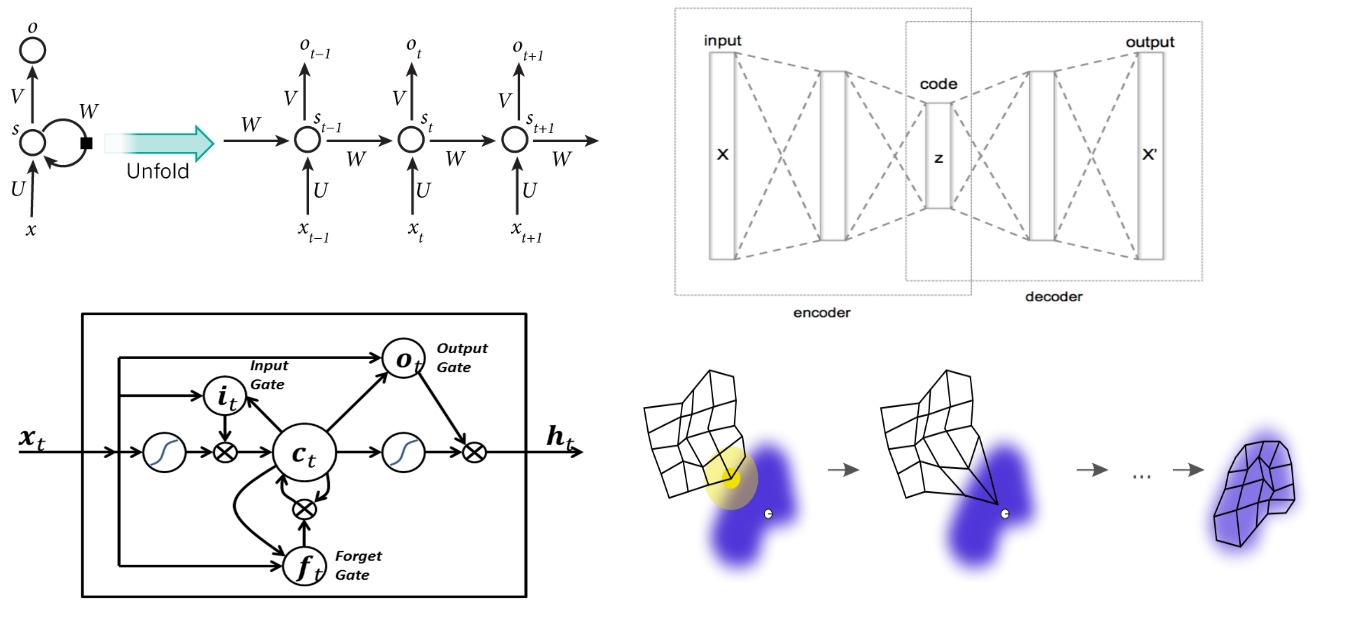
\includegraphics[scale=0.45]{figures/ANNs3}
    \caption{Representation of different neural network architectures. Top left shows an archetypal recurrent neural network, top right shows the idea behind autoencoders, bottom left is a long short-term block, the basic building block of long short-term memory and bottom right pictures the idea of self organising maps.}
    \label{fig:ANNs3}
\end{figure}

\subsection{Different Learning Methods}
So now that we have seen some different architectures let us take a look at some different learning techniques. 
%In discussing those we will use generic variables $x$ for parameters, i.e. weights and bias terms and $f$ for optimization objectives and explain how to apply them to the specifics of neural networks when not immediately apparent. 
Clearly we will need to adjust backpropagation or use completely different methods when dealing with architectures unlike feedforward networks. But what we want to take a quick look at are some variations of the very basic backpropagation algorithm we discussed above. To that point it should be noted that back propagation as a concept, i.e. that an error gets propagated from the output layer to the earlier layers, in no way relies on us using gradient descent. Therefore in addition to the obvious adjustments of learning rate we can drop gradient descent and instead use quasi-Newton methods, conjugate gradient methods as well as others.

\subsubsection{Dynamic Learning Rates and Momentum}

Nevertheless let us first take a look at learning rate adjustments. The general idea behind adjusting the rate dynamically is that we want to be able to take into account the shape of the error function, meaning that if the minimum lies in a ravine we might want a small learning rate so as to not overshoot the target, while, if we have a plateau relatively far from the minimum we want a higher learning rate in order to avoid getting stuck there for a long time. However since we do not know the shape of the error function beforehand and in fact both of the described propositions might be true we can not achieve this adaptiveness with a predetermined fixed learning rate (Figure \ref{fig:learning}). As a concrete example take the two functions 
\begin{align*}
    f_1(x)=x^2 \hspace{1cm}\mbox{ and }\hspace{1cm} f_2(x)=0.001x^2
\end{align*} 
and the two learning rates $\eta_1=\frac{1}{4}$ and $\eta_2=100$. We can easily see that both functions have their global minimum at $x^*=0$ and if we start gradient descent at the initial value $x_0=1$ in the case of $f_1$ we find that with $\eta_1$ we converge relatively quickly ($x_1=0.5$, $x_2=0.25$,...) while with $\eta_2$ we strongly diverge ($x_1=-199$, $x_2=39601$,...) so that $\eta_1$ is by far the better choice of learning rate. In the case of $f_2$, while we converge with both rates, $\eta_1$ will be far slower ($x_1=0.9995$, $x_2=0.99900025$,...) versus ($x_1=0.8$, $x_2=0.64$,...), so that $\eta_2$ would be the better choice. 

\begin{figure}
    \centering
    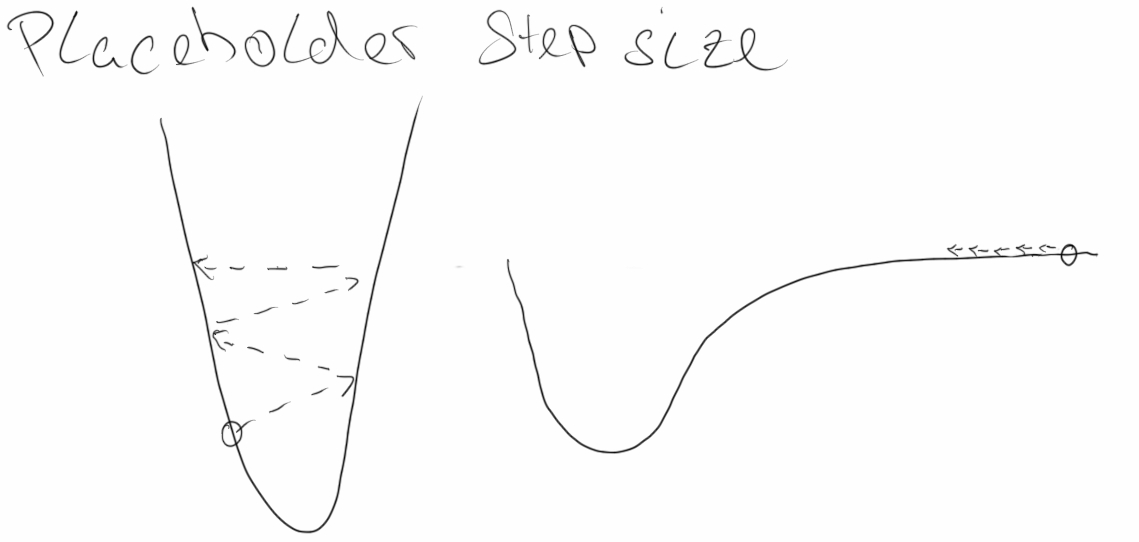
\includegraphics[scale=0.4]{figures/learning.jpg}
    \caption{Caption:TODO}
    \label{fig:learning}
\end{figure}

The most straight forward approach to solve this problem is to disregard the magnitude of the gradient completely and only considering the direction at each update step \cite{riedmiller1993direct}, which is the same as choosing a learning rate that is inversely proportional to the magnitude of the gradient, i.e.
$$\eta_t=\frac{\eta}{\Arrowvert\nabla f(x_t)\Arrowvert}$$
where $\eta$ is some constant factor essentially replacing the learning rate. This leads to update steps
$$x_{t+1}=x_t-\eta\frac{\nabla f(x_t)}{\Arrowvert\nabla f(x_t)\Arrowvert}$$
or in the one dimensional case
$$x_{t+1}=x_t-\eta \sign(\nabla f(x_t))$$
Another approach is to look for the best possible learning rate, i.e. to solve the line search problem
$$\eta_t=arg\min_{\eta\in\mathbbm{R}}f(x_t-\eta\nabla f(x_t))$$
In order to approximate this best rate we can use the a number of heuristics such as a backtracking line search or the Wolfe conditions \cite{wolfe1969convergence}. 

Another adjustment that can improve convergence in various ways is incorporating in the present weight update some influence of the past iterations and therefore adding a sort of momentum to the update procedure. If we denote by $\Delta x_t$ the update at time $t$, i.e.
$$x_{t+1}=x_t+\Delta x_t$$
then our new update rule will be
$$\Delta x_t=-\eta_t\nabla f(x_t)+\mu_t\Delta x_{t-1}$$
where $-\eta_t\nabla f(x_t)$ is the gradient descent step and $\mu_t$ is called the momentum parameter. By using momentum we can avoid oscillations in the error by averaging gradient components of opposing direction and accelerate convergence in long flat areas. Further in some cases it is possible to skip local minima as well as areas of little interest without performing minimization there.

Combination of these two general concepts now give rise to a multitude of different learning methods ranging from momentum based stochastic gradient descent \cite{bottou2012stochastic}
\begin{align*}
    \Delta x_t=\mu\Delta x_{t-1}-\eta\nabla f(x_t)
\end{align*}
to adaptive gradient methods such as 'AdaGrad' \cite{duchi2011adaptive} 
\begin{align*}
    (\Delta x_t)_i=-\eta\frac{(\nabla f(x_t))_i}{\sqrt{\sum_{t'=1}^t(\nabla f(x_{t'}))_i^2}}
\end{align*}
and 'Adam' \cite{kingma2014adam}
\begin{align*}
     (\Delta x_t)_i&=-\eta\frac{\sqrt{1-\mu_2}}{1-\mu_1}\frac{(\Phi_t)_i}{\sqrt{(\Psi_t)_i}+\varepsilon}\\
     \Phi_t&=\mu_1\Phi_{t-1}+(1-\mu_1)\nabla f(x_t)\\
     \Psi_t&=\mu_2\Psi_{t-1}+(1-\mu_2)(\nabla f(x_t))^2
\end{align*}
as well as many more \cite{tieleman2012lecture,zeiler2012adadelta,sutskever2013importance}.

\subsubsection{Conjugate Gradient Methods}

The 'pure' gradient descent method we just discussed adjusts the parameters in the steepest descent direction, i.e. the direction, in which the objective function decreases most rapidly. As we have already seen, in many cases choosing this direction might not allow for fast convergence. Above we used momentum in order to change this direction so that it takes into account the path we took to arrive at the current parameters. Conjugate gradient methods follow a similar approach, the general pattern being, that we calculate the current steepest descent, find a direction unlike past iteration directions along the steepest decent and update the parameters in that direction.

A short explanation of how this method is derived can be found in Appendix B, where we explore how conjugate directions are used to solve linear systems and how this is combined with gradient methods to solve minimization problems in quadratic functions. What we will discuss here is ways to implement the conjugate gradient idea for complex functions such as the error function in neural networks. Notation wise not much changes. We still have a function $f:\mathbbm{R}^n\rightarrow\mathbbm{R}$ which we want to minimize from an initial value $x_0$, however this time $f$ is not required to be quadratic. Instead we make the much less restrictive assumption, that the function is locally quadratic around the minimum, meaning we can find a second degree Taylor approximation close to the minimum. Given such a function and an initial value we will start as before, i.e. taking a step in the direction of steepest descent $d_0=-\nabla f(x_0)$, since no other information is available to us. Next we want to find the step size or learning rate to relate the terminology back to machine learning problems. Before we used 
$$c_k=\frac{\langle r_k, r_k\rangle}{\langle d_k,d_k\rangle_A}$$
but now there is no matrix $A$ available to us since the function does not have to be quadratic and even if it is $A$ would be unknown to us. There are now two option available to us. For the first we remember that the Hessian of the quadratic function used above is given by 
$$H_f(x)=A$$
so that that if we could find or at least approximate the Hessian of the new problem, it could be a good substitute for the calculation of the learning rate
$$c_k=\frac{\langle r_k, r_k\rangle}{d_k^TH_f(x_k)d_k}$$
In fact we do not even need the full Hessian but instead only the Hessian multiplied by a vector $H_f(x_k)d_k$ which as it turns out is relatively time and storage effective to calculate in neural networks \cite{pearlmutter1994fast}. This general approach leads to so called 'Hessian-free' learning which, while there seems to be very little research on the topic, appears to show some promise in deep learning \cite{martens2010deep}. Alternatively we could use one of the gradient based iterative approximation used in various Quasi-Newton methods, some of which we will discuss a bit later on. 

The second option we have to find the learning rate is to disregard our previous considerations to some degree and instead just look for the optimal learning rate 
$$c_k=arg\min_c{f(x_k+cd_k)}$$
via line search. In practice this is the preferred method even though a line search in complex optimization objectives such as neural networks can be very costly. In either way the algorithm is given by
\vspace{0.4cm}
\begin{algorithmic}
\State Step 1: Set $k=0$ and $d_0=-\nabla f(x_0)$
\vspace{0.3cm}
\State Step 2: Calculate $c_k$ either through line search or as $c_k=\frac{\langle \nabla f(x_k), \nabla f(x_k)\rangle}{d_k^TH_f(x_k)d_k}$
\vspace{0.3cm}
\State Step 3: Calculate $x_{k+1}=x_k+c_kd_k$
\vspace{0.3cm}
\State Step 3: Calculate $\beta_k=\frac{\langle \nabla f(x_{k+1}),\nabla f(x_{k+1})\rangle}{\langle \nabla f(x_{k}),\nabla f(x_{k})\rangle}$
\vspace{0.3cm}
\State Step 4: If $(k+1 \mbox{ mod } n)=0$ set $d_{k+1}=-\nabla f(x_{k+1})$ else set $d_{k+1}=-\nabla f(x_{k+1})+\beta_{k}d_{k}$ 
\vspace{0.3cm}
\State Step 5: $k\gets k+1$ and go to Step 2
\vspace{0.3cm}
\end{algorithmic}
\vspace{0.4cm}
until convergence. We reset the search directions every $n$ iterations since the amount of mutually conjugate directions in $\mathbbm{R}^n$ is bounded by $n$ and so after $n$ iterations subsequent iterations lose conjugacy which can lead to progress being halted until the direction is reset. One last thing to mention here is, that there are a number of different ways to choose $\beta_k$, all of which being equivalent in the case of quadratic functions. The one we used is known as the Fletcher-Reeves method, another example being Polak-Ribière which is given by
$$\beta_k=\frac{\langle-\nabla f(x_k),(-\nabla f(x_k)+\nabla f(x_{k-1})\rangle}{\langle \nabla f(x_{k-1}),\nabla f(x_{k-1})\rangle}$$
None of these is objectively better or worse across the board so that the question of which one to use is heavily problem dependent.

\subsubsection{Quasi-Newton Methods}
As a last learning approach we will take a quick look at Quasi-Newton methods. We remember that Newton's method lets us find roots of a real valued function $g$ by iterating
$$x_{k+1}=x_k-\frac{g(x_k)}{g'(x_k)}$$
and equivalently extrema of a function $f$ with $f'=g$. Similarly it is possible to find a minimum for multivariate functions if $f$ is locally quadratic around the minimum. We can see this by using the second order Taylor approximation at $x_k$ in direction $\Delta x$ where $f$ is given by
\begin{align*}
    f(x_k+\Delta x)&=f(x_k)+\Delta x^T \nabla f(x_k)+ \frac{1}{2}\Delta x^TH_f(x_k)\Delta x+O(\Arrowvert\Delta\Arrowvert^3)
\end{align*}
and finding the minimum with respect to $\Delta x$. Clearly if we could find this minimum, i.e. $\Delta x$ that solves $$\nabla_{\Delta x}f(x_k+\Delta x)=0$$ exactly, we would have found the minimum as $x^*=x_k+\Delta x$. However since this is the same problem as finding $x^*$ to begin with, that will not help us very much. What we will do instead is find a $\Delta x_k$ that minimizes the approximation 
\begin{align*}
    f(x_k+\Delta x_k)&\approx f(x_k)+\Delta x_k^T \nabla f(x_k)+ \frac{1}{2}\Delta x_k^TH_f(x_k)\Delta x_k
\end{align*}
While this approach does not give us $x^*$ directly, if we can solve it, what it does provide is a decent direction to search in which is all we need for a learning algorithm. To solve it as usual we have to find $\Delta x_k$ such that  
$$\nabla_{\Delta x_k}f(x_k+\Delta x_k)\approx\nabla f(x_k)+H_f(x_k)\Delta x_k=0$$
and therefore
$$H_f(x_k)\Delta x_k= -\nabla f(x_k)$$
This leaves us with two obvious options. We could solve the linear system approximately or invert $H_f(x_k)$ and calculate
$$\Delta x_k= -H^{-1}_f(x_k)\nabla f(x_k)$$
To solve the system approximately we could for example use conjugate gradient method or various other methods designed to solve linear equations. However since this is a moderately complex optimization problem (i.e. finding the Hessian and solving the linear equation) in every step of the overarching optimization problem, this approach is used rarely in high dimensional problems. This leaves us with inverting a high dimensional matrix, a problem which is equally as computationally expensive and would find little application in practice. 

Both of initial ideas being heavily flawed, Quasi-Newton methods offer a third solution. Instead of inverting the Hessian in each step we will find a reasonable approximation $H_k$ to the Hessian $H_f(x_k)$ which can be inverted with a lot less effort. In order to preserve the for our problem most important property of the Hessian we will choose $H_k$ so that it will satisfy the secant equation
$$\nabla f(x_{k-1})=\nabla f(x_k)-H_k\Delta x_{k-1}$$ 
Most of these methods use an iterative approach to approximating the Hessian in each step and then find the inverse, for which we will use the shorthand $B_k=H_k^{-1}$, using the Sherman-Morrison formula.
The algorithm then has the general form
\vspace{0.4cm}
\begin{algorithmic}
\State Step 1: Set $k=0$ and approximate some initial $B_0$ for example $B_0=I$
\vspace{0.3cm}
\State Step 2: Calculate $\Delta x_k=-\eta_kB_k\nabla f(x_k)$ using line search to find the step size
\vspace{0.3cm}
\State Step 3: Calculate $x_{k+1}=x_k+\Delta x_k$ and $B_{k+1}$
\vspace{0.3cm}
\State Step 4: $k\gets k+1$ and if convergence is not reached go to Step 2
\vspace{0.3cm}
\end{algorithmic}
\vspace{0.4cm}
There are plenty of methods to update $B_{k+1}$, to demonstrate one, the Broyden-Fletcher-Goldfarb-Shanno update \cite{roger1987practical} has the following shape
\begin{align*}
    B_{k+1}=\Large(I-\frac{\Delta x_k y_k^T}{y_k^T\Delta x_k}\Large)B_k\Large(I-\frac{y_k\Delta x_k^T}{y_k^T\Delta x_k}\Large)+\frac{\Delta x_k\Delta x_k^T}{y_k^T\Delta x_k}
\end{align*}
where $y_k=\nabla f(x_{k+1})-\nabla f(x_k)$.



\section{Convolutional Neural Networks}

So now that we have an idea how neural network function in general, we will explore a special kind of feedforward network called Convolutional Neural Network (ConvNet). Modern ConvNets consist of primarily of three different kinds of layers: Convolutional, Pooling and Fully-Connected. Additionally many ConvNets use layers of Rectified Linear Units in a particular fashion. We will now give a quick overview of the individual layers and then discuss different configurations and some practical concerns when describing the implementations we use. 


\subsection{Covolutional Layer}
First and foremost we have convolutional layers (Figure \ref{fig:layers} top). Each of these layers consist of a set of $K$ parameter tensors $W_k\in\mathbbm{R}^{F\times F\times D}$ called filters which are shared across neurons. The neurons in the layer are spatially arranged, so that adjacent neurons not only share parameters but also inputs. This is done in the following way. 

Assume the $l$th layer of the network is convolutional as described above getting as input a tensor 
$$X^{l-1}\in\mathbbm{R}^{H_{l-1}\times B_{l-1}\times D_{l-1}}$$ 
of $D_{l-1}$ feature maps $X^{l-1}_d\in\mathbbm{R}^{H_{l-1}\times B_{l-1}}$. The activation of this layer will again be a tensor 
$$X^{l-1}\in\mathbbm{R}^{H_{l}\times B_{l}\times D_{l}}$$ 
where each feature map is calculated as
$$X^{l}_k=X^{l-1}\otimes W_k$$
where $W_k$ is the $k-th$ filter and $\otimes$ is the convolutional operator
$$(X^{l-1}\otimes W)_{(n,m)}=\sum_{d=1}^{D_{l-1}} \sum_{i=0}^{F-1} \sum_{j=0}^{F-1} (X^{l-1}_d)_{(n+i,m+j)}W^d_{(i,j)}$$
which can be seen as sliding each filter across the height and width of the input map. The dimensions of the activation therefore are 

\begin{figure}
    \centering
    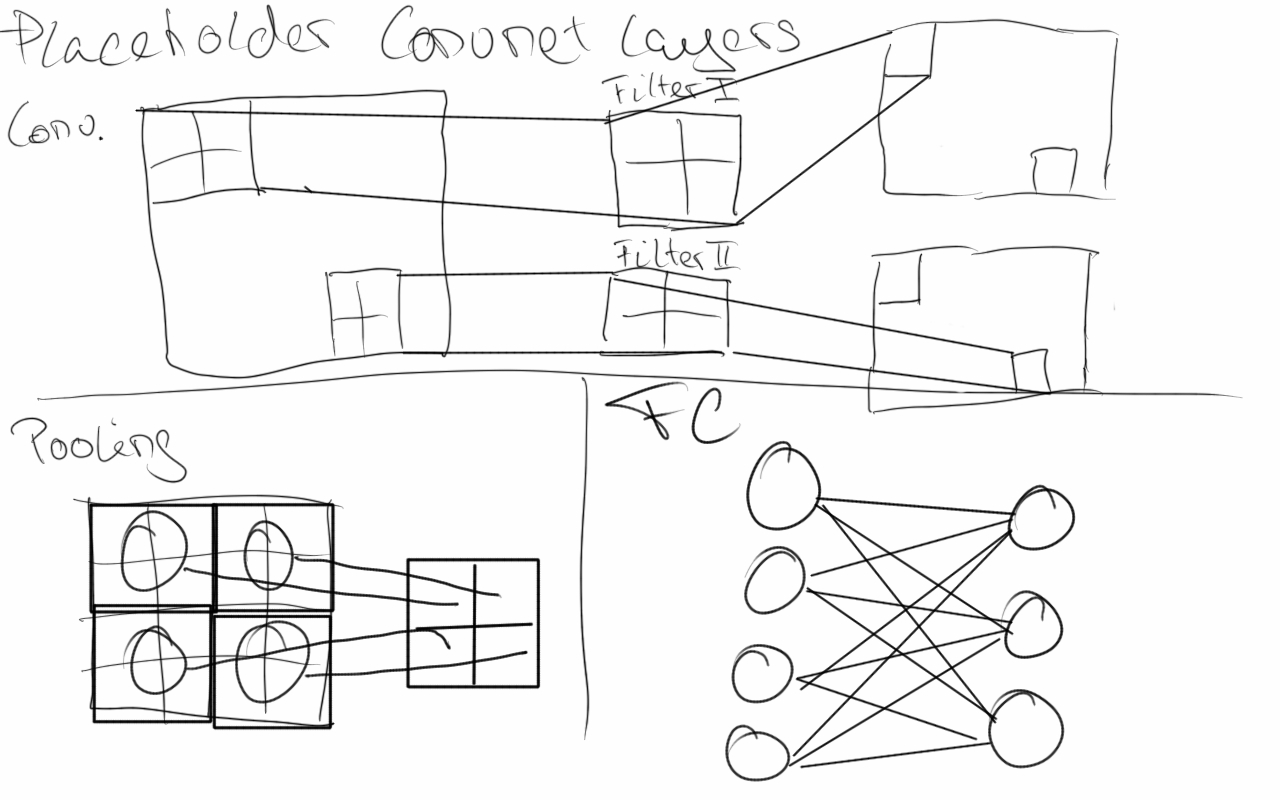
\includegraphics[scale=0.5]{figures/layers.jpg}
    \caption{Caption: TODO}
    \label{fig:layers}
\end{figure}

\begin{itemize}
    \item $H_l=H_{l-1}-F$ and $B_l=B_{l-1}-F$
    \item $D_l=K$
\end{itemize}
so that we need $(H_{l-1}-F)\cdot(B_{l-1}-F)\cdot K$ neurons and $F\cdot F\cdot K\cdot D$ parameters. If we compare this to regular feed forward layers (fully-connected layers below) the same amount of neurons would need on the order of $H_{l-1}^2\cdot B_{l-1}^2\cdot K\cdot D$ parameters. Convolution with these filters therefore allows us to recognize spacial patterns in a $F\times F$ window while drastically reducing the amount parameters and computation. 

One other thing that is often introduced to limit parameters and computation is the concept of striding, i.e. skipping the filter across the height and depth of the input map instead of sliding it across. In practice this means we get
$$(X^{l}_k)_{(n,m)}=(X^{l-1}\otimes W_k)_{S(n-1)+1,S(m-1)+1}$$
so that only about $\frac{1}{S^2}$ of the information is used and the rest is discarded. Something very similar can be achieved using pooling layers.



\subsection{Pooling Layer}
In ConvNets spatial pooling, i.e. taking a $n\times n$ window of inputs and combining them into a single output (Figure \ref{fig:layers} bottom left), is used to reduce the dimensionality of feature maps, thus reducing the number of parameters and the amount of computation in the network. The most common form of pooling used in ConvNets is max pooling, where we output the maximal input and discard the rest. This is often done in a max pooling layer with a $2\times2$-filter and a stride of $2$ across depth, effectively reducing the size of the representation by $75\%$. Aside from max pooling there are a number of other possible strategies such as average or sum pooling which are used much less frequently. Other than reducing the number of parameters and the amount of computation, pooling also helps making the network invariant to small distortions and to the scale of elements in the input.

\subsection{Fully-Connected Layer}
Fully-Connected (FC) layers are the layers used in regular feedforward networks described above (Figure $\ref{fig:layers}$ bottom right). Every neuron in the previous layer is connected to every neuron in the present layer and each of those connections is assigned its own weight parameter. 

\subsection{Rectified Linear Units}
Additionally to the layers mentioned above, many ConvNets make use of layers containing rectified linear units (ReLU). Rectified linear units are neurons which apply the rectifier activation function 
$$f(x)=\max(0,x)$$
In the case of ConvNets, ReLUs are used to replace activation functions in the previous layer, meaning that they are connected to only a single previous neuron and apply the rectifier function to the activation of that neuron. Theoretically we could incorporate this layer into the previous one by using the activation function there, however for the sake of clarity and comprehensibility it is often its own layer.
The main benefit of using the rectifier function as the activation function as opposed to for example a sigmoid function, is that its gradient $f'(x)$ does not vanish for large $x$ like the gradient of the sigmoid function does. In fact the gradient is locally constant either one or zero which makes computation easier and adds sparsity to gradients and activations.

There are variations of ReLUs which are used in some networks such as noisy ReLUs which include Gaussian noise to the output
$$f(x)=\max(0,x+Y) \mbox{, with }Y\sim N(0,\sigma^2(x))$$
or exponential linear units (ELUs)
\begin{align*}
    f(x)=\begin{cases}x &\mbox{if }x\geq 0\\
    a(e^x-1)&\mbox{otherwise}\end{cases}
\end{align*}
with hyper-parameter $a\geq0$.

\newpage

\section{Implementation}

\begin{figure}
    \centering
    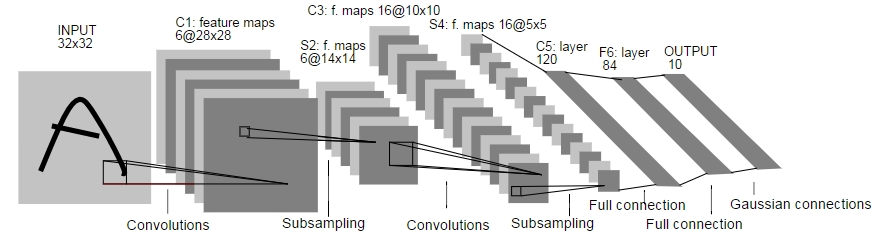
\includegraphics[scale=0.7]{figures/lenet}
    \caption{Caption}
    \label{fig:my_label}
\end{figure}

The most straightforward structure of a ConvNet begins with convolutional, ReLU and pooling layers. Each convolutional layer is followed by a ReLU layer and every one or two of these pairs is then followed by a pooling layer. After one or more iterations of this pattern we use combinations of fully-connected and ReLU layers and end on a fully-connected layer which should give us a representation of the objective, i.e. a label for classification and a value for regression. We thus have the following structure
$$\big[(Conv\rightarrow ReLU)^+\rightarrow Pool\big]^*\rightarrow (FC\rightarrow ReLU)^*\rightarrow FC\rightarrow\mbox{'Output'}$$
The basic idea behind this is that the convolutional layers learn to identify small spacial features such as edges and corners and the fully-connected layers combine the detected features into larger structures from which an output is generated.

There are of course all kinds of variations and some of the most successful networks in use right now are a lot more intricate than what we described here. We will explore some of those as we take a closer look at the architectures we employ to try and solve the central problem of this paper, but first let us take a closer look at the aforementioned problem.

\subsection{Problem Definition}

The task we want to automate is determining the rotation of a head given an image of it. To create a model we have a training set $\mathcal{D}$ consisting of $287390$ images and corresponding labels and two validation sets $\mathcal{V}_{\{1,2\}}$ of each $10000$ images and labels. In the sets each image is given in $128\times128$ greyscale (Fig. \ref{fig:data}a) and the labels are each three numbers signifying yaw pitch and roll of the head (Fig. \ref{fig:data}c). Before training we will do some additional pre-processing of the images, mainly by subtracting the mean (See Fig. \ref{fig:data}b) and scaling in a way so that all values lie in $[-1,1]$. 

\begin{figure}
    \centering
    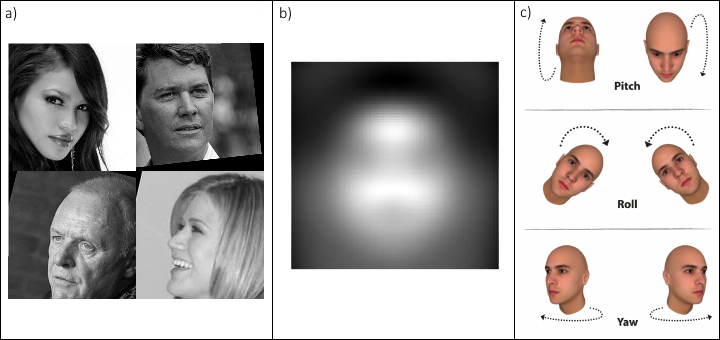
\includegraphics[scale=0.8]{figures/data.png}
    \caption{a) Examples of images in our dataset. b) Mean of images in the training set. c) Illustration of orientation of the head in terms of pitch , roll , and yaw taken from \cite{arcoverde2014enhanced}}.
    \label{fig:data}
\end{figure}

\subsection{A First ConvNet}

Our first ConvNet will follow the instructions for constructing a standard network as discussed above. We will keep the size of the network to a minimum as it will only serve as an introductory example and somewhat of a benchmark for the other models. The exact architecture can be viewed in Figure \ref{fig:net1}. As we can see, it will only use two convolutional layers, as well as one pooling and one FC layer. Certainly we will not expect great results, but it should suffice as a first point of reference. 

In contrast to the later networks we will also learn all the weights from scratch. The reasoning behind not doing this for the more intricate architectures is that we will use those that have already proven to be effective for similar tasks. Therefore, for these networks, there are already trained weights. Given, these weights are not trained for the exact task we want the network to accomplish, however as a starting off point in general they perform a lot better than completely random weights. This practice of taking pre-trained weights as an initial guess is known as fine-tuning and common practice when learning a ConvNet architecture.

\subsection{AlexNet}

The AlexNet architecture, as described in \cite{krizhevsky2012imagenet}, was the first substantial application of convolutional networks in computer vision. In structure it follows the simple rules outlined above with the one exception of normalization layers being added after convolutional layers (See Fig. \ref{fig:net2}).

\paragraph{Local Response Normalization}
The specific type of normalization is called local response normalization and its primary function is what is known as lateral inhibition. The term stems from neurobiology where it signifies the capacity of excited neurons to reduce the activity of its neighbors. In convolutional neural network architectures the term is used quite similarly. While there is no explicit concept of vicinity for neurons in convolutional layers, implicitly we will characterize vicinity by input region and normalize each activation by those in its neighborhood. This type of lateral inhibition achieves mainly two things for our network. It dampens activations in areas where they are uniformly large and strengthens signals in neighborhoods of small activations. Why exactly this is desirable is not fully understood, however empirically it reduces error rates when applied \cite{krizhevsky2012imagenet}.

\subsection{GoogLeNet}
GoogLeNet \cite{szegedy2014going} was the first successful convolutional network that significantly strayed from the sequential structure we describe above. Instead of just stacking layers, one after another, GoogLeNet's architecture uses so-called Inception Modules as its basic building block.

\begin{figure}
    \centering
    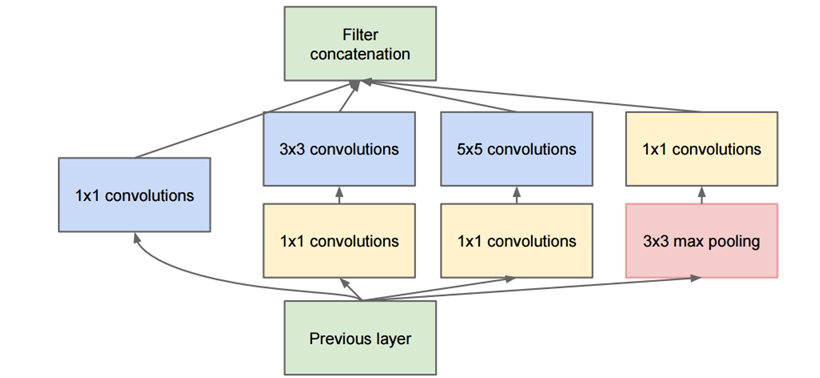
\includegraphics[scale=0.6]{figures/GoogLeNet3.png}
    \caption{Inception Module used in the GoogLeNet architectures.}
    \label{fig:inception}
\end{figure}


\paragraph{The Inception Module} The basic idea is that in sequential designs at each point where we decide between different size convolutions and pooling, we have little knowledge about which choice of layer will perform best. So instead of making a choice, which often came down to a best guess, with the 'Inception Module' we run multiple convolutions as well as pooling operations in parallel and then combine the distinct outputs into a single one. As we can see in Figure \ref{fig:inception} we are using filters of size $1,3,5$ (blue) and $3\times3$ max pooling (red). Additionally we are using convolutional layers of filter size $1$ (yellow) in order to reduce the depth of the input. This is done in order to increase performance, since just running the larger filters over the entire depth of the input is computationally expensive and takes a lot of parameters. As an example, if we have an input containing $100$ feature maps, a single convolutional layer with $20$ filters of size $5$ would need $50000$ parameters. If we instead preface this layer by a filter size $1$ convolutional layer of the same depth we will only need $12000$ parameters across both layers, $2000$ for the size $1$ layer and $10000$ for the size $5$ one, meaning we achieve about a $4$ times decrease in parameters and a decrease in computational complexity along the same line. Using this principle, GoogLeNet, despite seeming considerably larger, uses about $14$ times less parameters than AlexNet.

After computation is finished and all outputs volumes are generated, they are combined along depth by a concatenation layer. To make sure the height and width dimensions are identical across layers, all of the operations use a stride of $1$ and where it is needed, zero padding, i.e. adding zeros along the edges of the output in order to artificially increase size, is used.

\medskip\noindent
One other aspect of the original GoogLeNet architecture was that due to the depth, two auxiliary classifiers were added in order to amplify the gradient signal back through the network. However, with the introduction of batch normalization \cite{ioffe2015batch}, these classifiers have been ignored in more recent iterations.

\subsection{ResNet}
Here will be some theory about deep residual learning \cite{he2015deep}

\begin{figure}
    \centering
    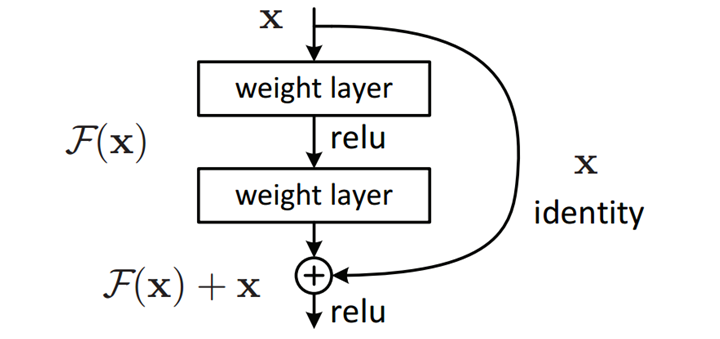
\includegraphics[scale=0.6]{figures/ResNet.png}
    \caption{Residual Block used in ResNet architectures.}
    \label{fig:res}
\end{figure}

\section{Results}










\newpage

\section{TODO}

\begin{itemize}
    \item Replace Learning Rate Figure
    \item Replace ConvNet Layer Figure
    \item Finish GoogLeNet/ResNet
    \item Figure for Inception Module, Residual Block
    \item Figure for all the networks (maybe Appendix or at the end somewhere)
    \item Finally get some results for the networks
    \item Find a way to reference ipython notebooks in a nice way
    \item (Maybe) Mention Batch Normalization
\end{itemize}










\newpage
\bibliographystyle{plain}
\bibliography{sample} 
\newpage






\appendix

\section{Perceptron}
Let $\mathcal{D}=\{(\mathbf{x}^i,y^i)\,|\,i=1,...,n\}$ be a dataset containing $n$ labeled labeled observations $y^i\in\{0,1\}$. As part of the family of linear classifiers the Perceptron algorithm searches for hyperplanes $$H_{(w,b)}=\{\mathbf{x}\,:\,\langle\mathbf{x},\mathbf{w}\rangle+b=0\}$$  
that separate the classes from each other. The particular condition Perceptron applies is simply that we find a hyperplane that separates these classes in such a way that the least amount is classified incorrectly. That means if we denote by 
\begin{align*}
    \sigma(\mathbf{x};\mathbf{w},b)=\begin{cases}0 &\mbox{if }\langle\mathbf{x},\mathbf{w}\rangle+b\leq0\\
    1&\mbox{otherwise}\end{cases}
\end{align*} 
the predicted label of $\mathbf{x}$ we want to find $\hat{\mathbf{w}}$ and $\hat{b}$ such that the $0/1$-loss 
$$\mathcal{L}_{0/1}(y,y')=1_{\{y=y'\}}$$ is minimized, i.e.
\begin{align*}
    (\hat{\mathbf{w}},\hat{b})&=arg\min_{(\mathbbm{w},b)}\sum_{i=1}^n\mathcal{L}_{0/1}(y^i,\sigma(\mathbf{x}^i;\mathbf{w},b))
\end{align*}
Now we want to find an iterative procedure to train such a classifier. Clearly we cannot use gradient descent, since neither the $0/1$-loss nor $\sigma$ are differentiable in the conventional way. To get around the $0/1$-loss not being differentiable we can simply use the fact that we have only two possible values for $y$, i.e. zero and one. This makes it relatively easy to use a different function, that has the same result for these two values. One possibility is the squared distance, i.e.
$$\mathcal{L}(y,y')=(y-y')^2$$ which is zero if both $y$ and $y'$ are equal and one if $y=1$ and $y'=0$ or vice versa. For simplicity we will also scale the new loss by $\frac{1}{2}$ which does not change the minimum but makes further calculations more coherent. With that now we have
\begin{align*}
    \frac{\partial\mathcal{L}}{\partial w_k}(y^i,\sigma(\mathbf{x}^i;\mathbf{w},b)))&=\big(y^i-\sigma(\mathbf{x}^i;\mathbf{w},b)\big)(-1)\frac{\partial\sigma}{\partial w_k}(\mathbf{x}^i;\mathbf{w},b)\\
    &=-\big(y^i-\sigma(\mathbf{x}^i;\mathbf{w},b)\big)\frac{\partial H}{\partial \alpha^i}(\alpha^i)x^i_k
\end{align*}
where $H$ is the Heaviside step function and $$\alpha^i=\langle \mathbf{x}^i,\mathbf{w}\rangle+b$$
Again, the Heaviside step function is not differentiable in the ordinary sense but its weak derivative is the Dirac delta function (distribution) so that in a sense the partial derivative is given by
\begin{align*}
    \frac{\partial\mathcal{L}}{\partial w_k}(y^i,\sigma(\mathbf{x}^i;\mathbf{w},b)))
    &=-\big(y^i-\sigma(\mathbf{x}^i;\mathbf{w},b)\big)x^i_k\delta(\alpha^i)
\end{align*}
Now some math which is beyond our discussion can show that if we just want the loss function to decrease and ignore certain complications such that the choice of $(\mathbf{w},b)=(\mathbf{0},0)$ does not span a hyperplane, we can disregard the delta function so that the update step can be written as
\begin{align*}
    \mathbf{w}^{k+1}=\mathbf{w}^{k}+\big(y^{k}-\sigma(\mathbf{x}^k;\mathbf{w}^k,b^k)\big)\mathbf{x}^{k}
\end{align*}
This is the same as writing
\begin{align*}
    \mathbf{w}^{k+1}=\begin{cases}
    \mathbf{w}^{k} &\mbox{if }\mathbf{x}^{k}\mbox{ is classified correctly}\\
    \mathbf{w}^{k}+\big(y^{k}-\sigma(\mathbf{x}^k;\mathbf{w}^k,b^k)\big)\mathbf{x}^{k+1}& \mbox{otherwise}
    \end{cases}
\end{align*}
which is the form most often seen in literature. Analogously we can find the update for $b_k$. 

\section{Conjugate Gradient}
In order to understand the conjugate gradient method let us take a few steps back and suppose we want to solve a much easier problem, namely the linear system
$$Ax=b$$
where $A\in\mathbbm{R}^{n\times n}$ is symmetric and positive definite. Such a matrix $A$ defines an inner product given by 
$$\langle \varphi,\psi\rangle_{A}=\varphi^TA\psi$$ 
and we say that the vectors $\varphi$ and $\psi$ are conjugate if they are orthogonal with respect to this inner product, i.e. $\langle \varphi,\psi\rangle_{A}=0$. Now let $\mathcal{D}=\{d_1,...,d_n\}$ be a set of $n$ non-zero vectors which are mutually conjugate, then $\mathcal{D}$ is a basis of $\mathbbm{R}^n$ so that for every vector $x_0$ we can find coefficients $c_i$ for which the solution $x^*$ of the linear equation is given by 
$$x^*=x_0+\sum_{i=1}^nc_i d_i$$
With $x_k=x_0+\sum_{i=1}^{k-1}c_i d_i$ we get that
\begin{align*}
    \langle d_k,x^*-x_k\rangle_A&=\sum_{i=k}^nc_i\langle d_k,d_i\rangle_A\\
    &=c_k\langle d_k,d_k\rangle_A
\end{align*}
and since
\begin{align*}
    \langle d_k,x^*-x_k\rangle_A&=\langle d_k, Ax^*-Ax_k\rangle\\
    &=\langle d_k, b-Ax_k\rangle
\end{align*}
we get
$$c_k=\frac{\langle d_k, b-Ax_k\rangle}{\langle d_k,d_k\rangle_A}$$
This means we can solve any such linear system by finding a set of conjugate directions $d_k$ and calculating the coefficients $c_k$ as described above. 

Now let us go one step further and assume we want to minimize a quadratic function
$$f(x)=\frac{1}{2}\Arrowvert \hat{A}x-\hat{b}\Arrowvert^2$$
for which $\hat{A}^T\hat{A}\in\mathbbm{R}^{n\times n}$ is positive definite. Clearly this problem admits a unique solution $x^*$ and we have 
$$\nabla f(x^*)=\hat{A}^T\hat{A}x^*-\hat{A}^T\hat{b}=0$$
which implies
$$\hat{A}^T\hat{A}x^*=\hat{A}^T\hat{b}$$
or with $A=\hat{A}^T\hat{A}$ and $b=\hat{A}^T\hat{b}$
$$Ax^*=b$$
so that we can, given an initial value $x_0$, find $x^*$ as follows:
\vspace{0.4cm}
\begin{algorithmic}
\State Step 1: Set $k=0$ and choose a random direction $d_0$
\vspace{0.3cm}
\State Step 2: Calculate $c_k=\frac{\langle d_k, b-Ax_k\rangle}{\langle d_k,d_k\rangle_{A}}$ and set $x_{k+1}=x_k+c_kd_k$
\vspace{0.3cm}
\State Step 3: $k\gets k+1$ 
\vspace{0.3cm}
\State Step 4: If $k=n$ then $x_k=x^*$ otherwise use Gram-Schmidt to calculate  $d_k$ conjugate to \phantom{Step 4: }$d_i$ for all $i<k$ and go to Step 2
\end{algorithmic}
\vspace{0.4cm}
 However this algorithm, while solving the problem in at most $n$ steps, has no way to guarantee that with each iteration we will get any closer to the solution and thus fails to deliver good approximations if we stop anywhere short of completion. Therefore this will clearly not make for an effective learning algorithm when we eventually want to generalize the approach to different, more complex problems. However if we combine this approach of finding conjugate directions with the idea of gradient descent we will get an effective algorithm, namely the conjugate gradient algorithm. 
 
So let us see how and why this algorithm works. First we will need some new notation. By $e_k$ we denote the error and by $r_k$ we will denote the residual at step $k$, i.e. $e_k=x_k-x^*$ and $r_k=b-Ax_k$. While the error indicates how far we are from the solution, the residual indicates how far we are from solving the equation. It is easy to see that 
\begin{align*}
    r_k&=Ax^*-Ax_k=-Ae_k \hspace{0.2cm}\mbox{ and}\\
    r_k&=-(Ax_k-b)=-\nabla f(x_k)
\end{align*}
meaning that $r_k$ is the direction of steepest descent at $x_k$. Given the initial value $x_0$ we do not have any prior information so the first step we take will be in the direction of steepest descent, i.e. 
$$d_0=r_0$$
Next we calculate $c_0$ as described above, i.e.
\begin{align*}
    c_0&=\frac{\langle d_0, b-Ax_0\rangle}{\langle d_0,d_0\rangle_A}\\
    &=\frac{\langle d_0, r_0\rangle}{\langle d_0,d_0\rangle_A}
\end{align*}
and set $x_1=x_0+c_0d_0$. Assuming now we have found $x_k$ and want to find $x_{k+1}$ in a direction conjugate to all directions taken before that is near the steepest descent. We can do this by projecting the residual onto the conjugate space, i.e.
$$\beta_{k,i}=\frac{\langle r_{k},d_i\rangle_{A}}{\langle d_i,d_i\rangle_{A}}$$
$$d_{k}=r_{k}-\sum_{i=0}^{k-1}\beta_{k,i}d_i$$
and then calculate the step size as described above
$$c_{k}=\frac{\langle d_k, r_k\rangle}{\langle d_k,d_k\rangle_A}$$
This still does not make for an efficient algorithm since we have to store all search directions and calculate multiple matrix multiplications in each step, however we can reformulate $d_k$ and $c_k$ as follows
\begin{align*}
    c_k&=\frac{\langle r_k,r_k\rangle}{\langle d_k,d_k\rangle_A}\hspace{1.3 cm}\mbox{ and}\\
    d_{k}&=r_{k}+\beta_{k-1}d_{k-1}\hspace{0.5 cm}\mbox{ with}\\
    \beta_k&=\frac{\langle r_{k+1},r_{k+1}\rangle}{\langle r_k,r_k\rangle}
\end{align*}
which requires the storage of only the last direction and residual and only a single matrix multiplication. Further, finding the conjugate search directions does not require $A$ which will come of use when generalizing the method.
In the proof of our above claim we will make use of the following short lemma.
\paragraph{Lemma 1}
For all $j<k$ we have $\langle r_{k},d_j\rangle=0$.
\begin{proof}
Start with $k=1$ keeping in mind that $x_0=0$
\begin{align*}
    \langle r_{1},d_0\rangle&=\langle b-Ax_{1},d_0\rangle\\
    &=\langle b-Ax_0-Ac_0d_0,d_0\rangle\\
    &=\langle r_0,d_0\rangle-c_0\langle d_0,d_0\rangle_A\\
    &=\langle r_0,d_0\rangle-\frac{\langle d_0, r_0\rangle}{\langle d_0,d_0\rangle_A}\langle d_0,d_0\rangle_A\\
    &=0
\end{align*}
which proofs the basis. Now assume the claim to be true up to some $k$. It follows that
\begin{align*}
    \langle r_{k+1},d_j\rangle&=\langle b-Ax_{k+1},d_j\rangle\\
    &=\langle b-A(x_k+c_kd_k),d_j\rangle\\
    &=\langle r_k,d_j\rangle - c_k\langle d_k,d_j\rangle_A 
\end{align*}
If $j<k$ then the first addend is zero by the induction hypothesis and the second is zero because different search directions are conjugate. If $j=k$ we have
\begin{align*}
    \langle r_k,d_k\rangle - c_k\langle d_k,d_k\rangle_A&=\langle r_k,d_k\rangle - \frac{\langle r_k,d_k\rangle}{\langle d_k,d_k\rangle_A}\langle d_k,d_k\rangle_A\\
    &=0
\end{align*}
which completes the proof. 
\end{proof}

\noindent
So that now we can turn to the original claim.

\paragraph{Proposition 1} The update direction $d_k$ and step size $c_k$ can be reformulated in the following way
\begin{align*}
    c_k&=\frac{\langle r_k,r_k\rangle}{\langle d_k,d_k\rangle_A}\hspace{1.3 cm}\mbox{ and}\\
    d_{k}&=r_{k}+\beta_{k-1}d_{k-1}\hspace{0.5 cm}\mbox{ with}\\
    \beta_k&=\frac{\langle r_{k+1},r_{k+1}\rangle}{\langle r_k,r_k\rangle}
\end{align*}


\begin{proof}
For $c_k$ we have
\begin{align}
    c_k&=\frac{\langle d_k, r_k\rangle}{\langle d_k,d_k\rangle_A}\nonumber\\
    &=\frac{\langle r_{k}-\sum_{i=0}^{k-1}\beta_{k,i}d_i, r_k\rangle}{\langle d_k,d_k\rangle_A}\nonumber\\
    &=\frac{\langle r_{k},r_k\rangle-\sum_{i=0}^{k-1}\beta_{k,i}\langle d_i, r_k\rangle}{\langle d_k,d_k\rangle_A}\nonumber\\
    &=\frac{\langle r_k,r_k\rangle}{\langle d_k,d_k\rangle_A}
\end{align}
where Eq. (A.1) follows by Lemma 1. Next is $d_k$. For the proof we will be using the following calculations. For one we have
\begin{align}
    r_{k+1}&=b-Ax_{k+1}\nonumber\\
    &=b-A(x_k+c_kd_k)\nonumber\\
    &=r_k-c_kAd_k
\end{align}
which implies that
\begin{align}
    Ad_k&=\frac{1}{c_k}(r_k-r_{k+1})\nonumber\\
    &=\frac{\langle d_k,d_k\rangle_A}{\langle r_k,r_k\rangle}(r_k-r_{k+1})
\end{align}
Further
\begin{align*}
    \langle d_k,d_k\rangle_A&=\langle d_k,r_k-\sum_{i=0}^{k-1}\beta_{k,i}d_i\rangle_A\\
    &=\langle d_k,r_k\rangle_A
\end{align*}
which in turn shows that
\begin{align}
    \langle r_{k+1},r_k\rangle &= \langle r_k-c_kAd_k,r_k\rangle\nonumber\\
    &=\langle r_k,r_k\rangle-c_k\langle d_k,r_k\rangle_A\nonumber\\
    &=\langle r_k,r_k\rangle-\frac{\langle r_k,r_k\rangle}{\langle d_k,d_k\rangle_A}\langle d_k,r_k\rangle_A\nonumber\\
    &=0
\end{align}
And finally for $j<k$ with Lemma 1 and Eq. (A.2)
\begin{align*}
    0&=\langle r_{k+1},d_{j+1}\rangle\\
    &=\langle r_{k+1},r_{j+1}-\sum_{i=0}^j\beta_{j+1,i}d_i\rangle\\
    &=\langle r_{k+1},r_{j+1}\rangle\\
    &=\langle r_{k+1},r_j-c_jAd_j\rangle\\
    &=\langle r_{k+1},r_j\rangle-c_j\langle r_{k+1},d_j\rangle_A\\
    &=\langle r_{k+1},d_j+\sum_{i=0}^{j-1}\beta_{j+1,i}d_i\rangle-c_j\langle r_{k+1},d_j\rangle_A\\
    &=-c_j\langle r_{k+1},d_j\rangle_A
\end{align*}
so that
\begin{align}
    \langle r_{k+1},d_j\rangle_A=0
\end{align}
Now let us get to the proof. We have
\begin{align}
    d_{k+1}&=r_{k+1}-\sum_{i=0}^k\beta_{k+1,i}d_i\nonumber\\
    &=r_{k+1}-\sum_{i=0}^k\frac{\langle r_{k+1},d_i\rangle_{A}}{\langle d_i,d_i\rangle_{A}}d_i\nonumber\\
    &=r_{k+1}-\frac{\langle r_{k+1},d_k\rangle_{A}}{\langle d_k,d_k\rangle_{A}}d_k\\
    &=r_{k+1}-\frac{\langle r_{k+1},Ad_k\rangle}{\langle d_k,d_k\rangle_{A}}d_k\nonumber\\
    &=r_{k+1}-\frac{\langle d_k,d_k\rangle_A}{\langle r_k,r_k\rangle}\frac{\langle r_{k+1},r_k-r_{k+1}\rangle}{\langle d_k,d_k\rangle_{A}}d_k\\
    &=r_{k+1}+\frac{\langle d_k,d_k\rangle_A}{\langle r_k,r_k\rangle}\frac{\langle r_{k+1},r_{k+1}\rangle}{\langle d_k,d_k\rangle_{A}}d_k\\
    &=r_{k+1}+\frac{\langle r_{k+1},r_{k+1}\rangle}{\langle r_k,r_k\rangle}d_k\nonumber
\end{align}
Here Eq. (A.6) follows from Eq. (A.5), Eq. (A.7) from Eq. (A.3) and Eq. (A.8) from Eq. (A.4).
\end{proof}

\section{Backpropagation in ConvNets}

As in 'regular' feedforward networks, we can calculate gradients and thus parameter updates via backpropagation. Here we will go through each of the layers mentioned above and take a quick look at the essentials of error propagation as well as parameter derivatives where available. In other words for layer $l$ of any kind we will trace $$\boldsymbol{\delta}^{l-1}=\nabla_{\mathbf{x}^{l-1}}E(\mathbf{x}^L,y)$$
back to $\boldsymbol{\delta}^{l}$ and if the layer has parameters we also find 
$\nabla_{\mathbf{w}^l}E(\mathbf{x}^L,y)$
given $\boldsymbol{\delta}^{l}$.

\paragraph{Convolutional Layer} Let the $l$-th layer of a net be convolutional and let the $k$-th filter be labeled $W_k^l$. Then the partial derivative of the error with respect to the weight $(W_k^l)^d_{(i,j)}$ is given by
\begin{align*}
    \frac{\partial}{\partial(W_k^l)^d_{(i,j)}}E(\mathbf{x}^L,y)
    &=\sum_{n,m}\Big(\frac{\partial}{\partial (W_k^l)^d_{(i,j)}}  (X^l_k)_{(n,m)}\Big)\Big(\frac{\partial}{\partial (X^l_k)_{(n,m)}}E(\mathbf{x}^L,y)\Big)\\
    &=\sum_{n,m}\Big(\frac{\partial}{\partial (W_k^l)^d_{(i,j)}}  (X^{l-1}\otimes W_k^l)_{(n,m)}\Big)\Big(\frac{\partial}{\partial (X^l_k)_{(n,m)}}E(\mathbf{x}^L,y)\Big)\\
    &=\sum_{n,m}\Big(\frac{\partial}{\partial (W_k^l)^d_{(i,j)}}  \sum_{i',j',d'} (X^{l-1}_{d'})_{(n+i',m+j')}(W_k^l)^{d'}_{(i',j')}\Big)\Big(\frac{\partial}{\partial (X^l_k)_{(n,m)}}E(\mathbf{x}^L,y)\Big)\\
    &=\sum_{n,m} (X^{l-1}_{d})_{(n+i,m+j)}\Big(\frac{\partial}{\partial (X^l_k)_{(n,m)}}E(\mathbf{x}^L,y)\Big)
\end{align*}
and if we denote 
$$\delta_{k,n,m}^l=\frac{\partial}{\partial (X^l_k)_{(n,m)}}E(\mathbf{x}^L,y)$$
then 
\begin{align*}
    \frac{\partial}{\partial(W_k^l)^d_{(i,j)}}E(\mathbf{x}^L,y)&=\sum_{n,m} (X^{l-1}_{d})_{(n+i,m+j)}\delta_{k,n,m}^l
\end{align*}
Similarly we have
\begin{align*}
    \delta_{k',n',m'}^{l-1}
    &=\frac{\partial}{\partial (X^{l-1}_{k'})_{(n',m')}}E(\mathbf{x}^L,y)\\
    &=\sum_{n,m,k}\Big(\frac{\partial}{\partial (X^{l-1}_{k'})_{(n',m')}}(X^l_k)_{(n,m)}\Big)\delta_{k,n,m}^l\\
    &=\sum_{n,m,k}\Big(\frac{\partial}{\partial (X^{l-1}_{k'})_{(n',m')}}(X^{l-1}\otimes W_k^l)_{(n,m)}\Big)\delta_{k,n,m}^l\\
    &=\sum_{n,m,k}\Big(\frac{\partial}{\partial (X^{l-1}_{k'})_{(n',m')}}\sum_{i,j,d} (X^{l-1}_{d})_{(n+i,m+j)}(W_k^l)^{d}_{(i,j)}\Big)\delta_{k,n,m}^l
\end{align*}
so that for those $i',j'$ for which $(n'-i',m'-j')\in[1,H_l]\times[1,B_l]$ we have
\begin{align*}
    \delta_{k',n',m'}^{l-1}=\sum_k\sum_{i',j'}(W_k^l)^{k'}_{(i',j')}\delta_{k,n'-i',m'-j'}^l
\end{align*}
\paragraph{ReLU Layer}
Let the $l$-th layer be a ReLU layer and let $x^{l-1}_i$ be the activation from the preceding layer used in neuron $i$. Then 
$$x^l_i=\sigma(x^{l-1}_i)=\max(0,x^{l-1}_i)$$
and thus 
\begin{align*}
    \delta_i^{l-1}&=\sigma'(x^{l-1}_i)\delta_i^{l}\\
    &=1_{\big\{x^{l-1}_i>0\big\}}\delta_i^{l}
\end{align*}
\paragraph{Pooling Layer}
Let the $l$-th layer be a max pooling layer then for the appropriate $i',j'$ we have $$(X^l_d)_{(n,m)}=\max_{i',j'}(X^{l-1}_d)_{(i',j')}$$
so that similarly to the ReLU example we have
\begin{align*}
    \delta^{l-1}_{i,j,d}=1_{\big\{i,j=arg\max_{i',j'}(X^{l-1}_d)_{(i',j')}\big\}}\delta^{l}_{n,m,d}
\end{align*}
Applying this to different pooling layers such as average or sum pooling is rather straight forward and will therefore not be discussed here.
\paragraph{Normalization Layer}






\end{document}

